% -- Encoding UTF-8 without BOM
% -- XeLaTeX => PDF (BIBER)

\documentclass[english]{cv-style}

\usepackage{graphicx}

\begin{document}

\header{Rizki }{Mufrizal}
%\lastupdated

%----------------------------------------------------------------------------------------
% SIDEBAR SECTION  -- In the aside, each new line forces a line break
%----------------------------------------------------------------------------------------
\begin{aside}
\section{.}
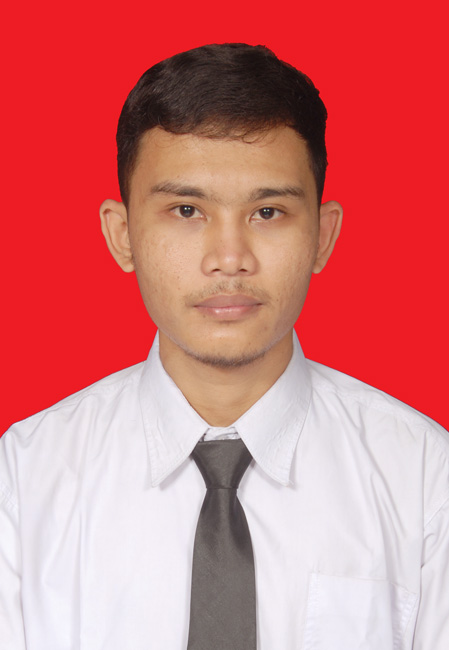
\includegraphics[width=4cm]{foto}
%
\section{Personal Info}
15 November, Puuk
%
\section{Contact Info}
+685359061036
mufrizalrizki@gmail.com
https://rizkimufrizal.github.io
RizkiMufrizal (Github)
RizkiMufrizal (LinkedIn)
~
Jl. Raya Haji Muhammad Tohir Gang Kapuk 32 RT 002/001, Beji, Pondok Cina, 16424, Depok, Indonesia
%
\end{aside}
%----------------------------------------------------------------------------------------
% WORK EXPERIENCE SECTION
%----------------------------------------------------------------------------------------
\section{Work Experience}
  \vspace{-0.3cm}
\begin{entrylist}
%------------------------------------------------
\entry
  {\scalebox{.6}[1.0]{Jan 2014 - Nov 2015}}
  {Assistant of Accounting Laboratory Advanced A}
  {Gunadarma University}
  {As a developer of the development of accounting learning modules}
%------------------------------------------ ------
\entry
  {\scalebox{.6}[1.0]{Nov 2015 - Oct 2016}}
  {Senior Assistant of Technical Information Laboratory}
  {Gunadarma University}
  {As responsibility of software engineering practicum 2, human and computer interaction, network programming and fixed assistant of informatics engineering laboratory Gunadarma University}
%------------------------------------------------
\entry
  {\scalebox{.6}[1.0]{Nov 2016 - Jan 2017}}
  {Back End Developer}
  {PT. TaniHub Indonesia}
  {\vspace{-0.3cm}
  \begin{itemize}\small{
    \item Develop Web Application Client using Node.js and Express.js.
    \item Develop REST API for version 1 using Node.js and Express.js.}
  \end{itemize}}
%------------------------------------------------
\entry
  {\scalebox{.6}[1.0]{Feb 2017 - Jun 2017}}
  {Software Engineer}
  {PT. TaniHub Indonesia}
  {\vspace{-0.3cm}
  \begin{itemize}\small{
    \item Develop REST API for Version 1 using Node.js and Express.js.
    \item Develop REST API and OAuth2 for Version 2 using Node.js and Express.js.
    \item Develop Web Application Admin Dashboard using Angular JS.
    \item Develop Web Application Retail Dashboard using Angular 4.
    \item Develop iOS Application using Xcode.}
  \end{itemize}}
%------------------------------------------------
\entry
  {\scalebox{.6}[1.0]{Jul 2017 - Present}}
  {API Consultant}
  {PT. Emerio Indonesia}
  {\vspace{-0.3cm}
  \begin{itemize}\small{
    \item Implements API Gateway Using Axway.
    \item Development Policy Using Policy Studio Axway.
    \item Research And Development Jenkins And Gitlab.
    \item Implements Data Center And Data Recovery Using Cassandra.
    \item Implements Master Slave MySQL/MariaDB.
    \item Implements Custom Security Like HMAC And OAuth2.
    \item Research And Development 3Scale API Gateway (Red Hat).
    \item Research And Development Tyk API Gateway.}
  \end{itemize}}
%------------------------------------------------
\end{entrylist}
%----------------------------------------------------------------------------------------
% EDUCATION SECTION
%----------------------------------------------------------------------------------------
\section{Education}
  \vspace{-0.3cm}
\begin{entrylist}
%------------------------------------------------
\entry
{\scalebox{.8}[1.0]{2006 - 2009}}
{Natural Science}
{MTsS Jeumala Amal, Lueng Putu, Indonesia}
{}
%------------------------------------------------
\entry
{\scalebox{.8}[1.0]{2009 - 2012}}
{Natural Science}
{MAS Jeumala Amal, Lueng Putu, Indonesia}
{}
%------------------------------------------------
\entry
{\scalebox{.8}[1.0]{2012 - 2016}}
{Technical Information}
{Gunadarma University, Depok, Indonesia}
{}
%------------------------------------------------
\entry
{\scalebox{.8}[1.0]{2016 - Present}}
{Information System Software}
{Gunadarma University, Jakarta, Indonesia}
{}
%------------------------------------------------
\end{entrylist}
\vspace{-0.3cm}

\section{Skill}
\vspace{-0.3cm}
\begin{itemize}
\item Java Programming
\item Kotlin Programming
\item JavaScript Programming
\item Swift Programming
\item PHP Programming
\item Ruby Programming
\item Spring Framework
\item Hibernate Framework
\item Angular JS
\item Angular 4
\item Node JS
\item Express JS
\item Sails JS
\item Linux
\item Windows
\item OSX
\item Policy Axway
\item API Gateway Axway
\item Apache Cassandra
\item Docker
\end{itemize}
%----------------------------------------------------------------------------------------
% INTERESTS SECTION
%----------------------------------------------------------------------------------------3
\section{Certifications}
\vspace{-0.3cm}
\begin{entrylist}
%--------------------------------------------
\entry
{\scalebox{.8}[1.0]{Feb 2015 - Present}}
{MTA Database Administration Fundamentals}
{Microsoft}
{}
%--------------------------------------------
\entry
{\scalebox{.8}[1.0]{Nov 2016 - Present}}
{Using Node.js with Visual Studio Code}
{Microsoft}
{}
%--------------------------------------------
\entry
{\scalebox{.8}[1.0]{Nov 2016 - Present}}
{Shaping up with Angular.js}
{Code School}
{}
%--------------------------------------------
\entry
{\scalebox{.8}[1.0]{Nov 2016 - Present}}
{NDG Linux Essentials}
{Cisco Networking Academy}
{}
%--------------------------------------------
\end{entrylist}
\section{Publications}
\vspace{-0.2cm}
\begin{entrylist}
%--------------------------------------------
\entry
{\scalebox{.8}[1.0]{1 Sep 2015}}
{Implementasi Arsitektur REST API Pada Perpustakaan XYZ Berbasis Framework Spring MVC Dan Hibernate}
{}
{This writing contains the architecture of one type of web service that is REST (Representational State Transfer), response request http and CORS (Cross Origin Resource Sharing)}
%--------------------------------------------
\entry
{\scalebox{.8}[1.0]{1 Jan 2016}}
{Ebook Hibernate Spring}
{}
{Ebook hibernate spring serves as a learning material for the responsible eyes of software engineering practicum 2 in the laboratory of informatics engineering Gunadarma University}
%--------------------------------------------
\end{entrylist}

\section{Projects}
\vspace{-0.3cm}
\begin{entrylist}
%--------------------------------------------
\entry
{\scalebox{.6}[1.0]{Jul 2017 - Dec 2017}}
{API Gateway With Axway At PermataBank}
{}
{}
%--------------------------------------------
\entry
{\scalebox{.6}[1.0]{Aug 2017 - Dec 2017}}
{Apache Cassandra Data Center And Data Recovery At BTPN}
{}
{}
%--------------------------------------------
\entry
{\scalebox{.6}[1.0]{Mei 2017 - Jun 2017}}
{Absensi PT. Graha Usaha Teknik Development}
{}
{}
%--------------------------------------------
\entry
{\scalebox{.6}[1.0]{Mei 2017 - Jun 2017}}
{TaniHub Tani Retail Development}
{}
{}
%--------------------------------------------
\entry
{\scalebox{.6}[1.0]{Jan 2017 - Mei 2017}}
{TaniHub API Version 2 Development}
{}
{}
%--------------------------------------------
\entry
{\scalebox{.6}[1.0]{Mar 2017 - Mei 2017}}
{TaniHub iOS Development}
{}
{}
%--------------------------------------------
\entry
{\scalebox{.6}[1.0]{Mar 2016 - Mei 2016}}
{Koperasi Syariah Srengseng Sawah}
{}
{}
%--------------------------------------------
\end{entrylist}
\end{document}